\documentclass{beamer}
\usetheme{Madrid}
\usecolortheme{whale}
\usepackage{graphicx}
\usepackage{amsmath}
\usepackage{hyperref}
\usepackage{tikz}

\title{Security Implications of Asset Management}
\subtitle{Hardware, Software, and Data Security}
\author{Cybersecurity Fundamentals}
\date{\today}

\begin{document}

\begin{frame}
\titlepage
\end{frame}

\begin{frame}
\frametitle{The Asset Security Lifecycle: Why Management Matters}
\begin{itemize}
\item \textbf{Asset management} is the systematic process of deploying, operating, maintaining, and disposing of assets securely.
\item Every piece of hardware, software, and data has security implications throughout its entire lifecycle.
\item Proper asset management reduces the risk of unauthorized access, data breaches, and compliance violations.
\item Organizations without formal asset management procedures face significantly higher security risks.
\end{itemize}

\begin{block}{The Asset Lifecycle}
Acquisition → Assignment → Monitoring → Disposal
\end{block}
\end{frame}

\begin{frame}
\frametitle{Security Begins Before Purchase: Acquisition \& Procurement Basics}
\begin{itemize}
\item \textbf{Procurement} is the process of selecting and obtaining assets with security requirements in mind.
\item Security standards must be established before purchase to avoid introducing vulnerabilities into your organization.
\item Security features should be included in the requirements specification for any hardware or software acquisition.
\item Verify that manufacturers and vendors follow secure development and manufacturing practices.
\end{itemize}

\begin{alertblock}{Security Question}
Always ask: "What security controls are built into this product, and how will they integrate with our existing security infrastructure?"
\end{alertblock}
\end{frame}

\begin{frame}
\frametitle{Vendor Security Assessment: Choosing Trustworthy Partners}
\begin{itemize}
\item \textbf{Vendor assessment} evaluates potential suppliers based on their security practices and reliability.
\item Third-party vendors with weak security practices can create backdoors into your systems.
\item Request documentation of security certifications and compliance with industry standards (e.g., ISO 27001).
\item Evaluate the vendor's history of responding to security vulnerabilities and issuing patches.
\end{itemize}

\begin{exampleblock}{Vendor Red Flags}
\begin{itemize}
\item No security contact information
\item Poor patch response history
\item Unwillingness to share security documentation
\item Unclear data handling practices
\end{itemize}
\end{exampleblock}
\end{frame}

\begin{frame}
\frametitle{Total Cost of Secure Ownership: Budget Planning for Security}
\begin{itemize}
\item \textbf{Total cost of secure ownership (TCSO)} includes all expenses related to securely maintaining an asset.
\item Security costs extend beyond the initial purchase price to include ongoing maintenance, updates, and secure disposal.
\item Cutting corners on security features during procurement often leads to higher costs later due to breaches or remediation.
\item Budget for security training for users who will interact with the new assets.
\end{itemize}

\begin{table}
    \small
\begin{tabular}{|l|l|}
\hline
\textbf{Initial Costs} & \textbf{Ongoing Costs} \\
\hline
Purchase price & Security updates \\
Security setup & Monitoring tools \\
Implementation & Security testing \\
Configuration & Secure disposal \\
\hline
\end{tabular}
\end{table}
\end{frame}

\begin{frame}
\frametitle{From Delivery to Deployment: Secure Receiving Processes}
\begin{itemize}
\item \textbf{Secure receiving} ensures new assets are verified, documented, and protected upon arrival.
\item Verify that delivered hardware matches exactly what was ordered to prevent supply chain attacks.
\item Check the integrity of software packages by comparing checksums and verifying digital signatures.
\item Create a secure staging environment to test and configure new assets before adding them to your network.
\end{itemize}

\begin{center}
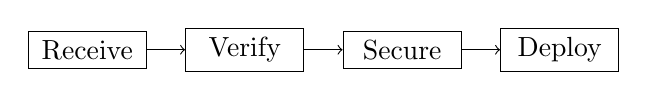
\begin{tikzpicture}[node distance=2cm]
\node (receive) [draw, rectangle, minimum width=1.5cm] {Receive};
\node (verify) [draw, rectangle, minimum width=1.5cm, right of=receive] {Verify};
\node (secure) [draw, rectangle, minimum width=1.5cm, right of=verify] {Secure};
\node (deploy) [draw, rectangle, minimum width=1.5cm, right of=secure] {Deploy};
\draw[->] (receive) -- (verify);
\draw[->] (verify) -- (secure);
\draw[->] (secure) -- (deploy);
\end{tikzpicture}
\end{center}
\end{frame}

\begin{frame}
\frametitle{Who Owns What? Asset Assignment \& Responsibility}
\begin{itemize}
\item \textbf{Asset ownership} establishes who is responsible for the security of each organizational asset.
\item Proper assignment of assets creates clear accountability for maintaining security controls.
\item Every asset should have a designated owner who understands their security responsibilities.
\item Document the assignment process with signatures acknowledging security policies and acceptable use.
\end{itemize}

\begin{block}{Asset Owner Responsibilities}
\begin{enumerate}
\item Ensure proper security controls are in place
\item Authorize access to the asset
\item Review security status regularly
\item Report security incidents promptly
\end{enumerate}
\end{block}
\end{frame}

\begin{frame}
\frametitle{Classification Fundamentals: Identifying Critical Assets}
\begin{itemize}
\item \textbf{Asset classification} is the process of categorizing assets based on their sensitivity and importance.
\item Classification helps determine appropriate security controls and handling procedures for each asset.
\item Improper classification can lead to either inadequate protection or wasteful security spending.
\item Classification should be reviewed periodically as the value and sensitivity of assets may change over time.
\end{itemize}

\begin{alertblock}{Common Classification Levels}
\begin{description}
\item[Public] Information that can be freely disclosed
\item[Internal] Information for use within the organization only
\item[Confidential] Sensitive information requiring protection
\item[Restricted] Highly sensitive information with strictly controlled access
\end{description}
\end{alertblock}
\end{frame}

\begin{frame}
\frametitle{Data Sensitivity Levels: From Public to Strictly Confidential}
\begin{itemize}
\item \textbf{Data sensitivity} refers to the potential harm that could result from unauthorized disclosure or access.
\item Different types of data require different security controls based on their sensitivity level.
\item Personally identifiable information (PII) and financial data typically require higher levels of protection.
\item The sensitivity level should dictate encryption requirements, access controls, and monitoring intensity.
\end{itemize}

\begin{table}
\begin{tabular}{|l|l|l|}
\hline
\textbf{Sensitivity} & \textbf{Example Data} & \textbf{Protection Required} \\
\hline
Low & Marketing materials & Basic controls \\
Medium & Internal documents & Access controls \\
High & Customer information & Encryption, logging \\
Critical & Financial records & Strict access, auditing \\
\hline
\end{tabular}
\end{table}
\end{frame}

\begin{frame}
\frametitle{Hardware Classification: Securing Physical Devices}
\begin{itemize}
\item \textbf{Hardware classification} categorizes physical devices based on their criticality to operations and security risks.
\item Critical infrastructure hardware (servers, firewalls) requires the highest security classification and protection.
\item End-user devices should be classified based on the sensitivity of data they can access or store.
\item Hardware that processes sensitive information may require special handling procedures and physical security measures.
\end{itemize}

\begin{exampleblock}{Example: Hardware Classification Matrix}
\begin{description}
\item[Class A] Critical infrastructure (core servers, network devices)
\item[Class B] Business operations systems (departmental servers, workstations)
\item[Class C] End-user devices (standard laptops, desktops)
\item[Class D] Peripheral devices (printers, scanners)
\end{description}
\end{exampleblock}
\end{frame}

\begin{frame}
\frametitle{Software Classification: Managing Application Security Risks}
\begin{itemize}
\item \textbf{Software classification} identifies applications based on their security impact and business value.
\item Software that handles sensitive data or has privileged system access requires stricter security controls.
\item Operating systems and security applications typically receive the highest classification due to their critical functions.
\item Unauthorized or unapproved software (shadow IT) presents significant security risks and should be identified.
\end{itemize}

\begin{block}{Software Risk Factors}
    \small
\begin{itemize}
\item Access to sensitive data
\item System privileges required
\item Network connectivity needed
\item Public exposure
\item Update/patch availability
\end{itemize}
\end{block}
\end{frame}

\begin{frame}
\frametitle{Asset Tracking 101: Why We Monitor Our Digital Property}
\begin{itemize}
\item \textbf{Asset tracking} is the continuous process of monitoring the location, status, and security of organizational assets.
\item Without proper tracking, organizations cannot detect missing assets or unauthorized changes to their systems.
\item Effective tracking enables rapid response to security incidents by identifying affected assets quickly.
\item Automated asset tracking tools can continuously monitor for changes and alert security teams to unusual activity.
\end{itemize}

\begin{alertblock}{Security Benefits of Asset Tracking}
Asset tracking allows organizations to:
\begin{itemize}
\item Identify unauthorized devices on the network
\item Detect missing or stolen equipment
\item Ensure compliance with security policies
\item Accelerate security incident response
\end{itemize}
\end{alertblock}
\end{frame}

\begin{frame}
\frametitle{Inventory Management: Tools \& Techniques for Accurate Counts}
\begin{itemize}
\item \textbf{Inventory management} involves maintaining an accurate database of all hardware, software, and data assets.
\item Regular inventory audits compare physical and digital assets against records to identify discrepancies.
\item Automated discovery tools can identify hardware and software assets connected to the network.
\item RFID tags and barcodes can help track physical assets throughout their lifecycle.
\end{itemize}

\begin{table}
    \scriptsize
\begin{tabular}{|l|p{5cm}|}
\hline
\textbf{Inventory Method} & \textbf{Best For} \\
\hline
Manual counting & Small organizations, high-security environments \\
Barcode scanning & Physical asset tracking, moderate scale deployments \\
RFID tracking & Large organizations, automated asset movement detection \\
Network scanning & Software inventory, detecting unauthorized devices \\
\hline
\end{tabular}
\end{table}
\end{frame}

\begin{frame}
\frametitle{Network Enumeration: Identifying Every Connected Device}
\begin{itemize}
\item \textbf{Network enumeration} is the process of identifying and cataloging all devices connected to a network.
\item Regular enumeration helps detect unauthorized devices that could represent security threats.
\item Enumeration tools scan IP ranges to discover active hosts and determine what services they're running.
\item Comparing enumeration results against the authorized inventory helps identify security gaps.
\end{itemize}

\begin{exampleblock}{Basic Enumeration Process}
\begin{enumerate}
\item Scan network ranges for active hosts
\item Identify operating systems and services
\item Compare results to authorized inventory
\item Investigate and remediate discrepancies
\end{enumerate}
\end{exampleblock}
\end{frame}

\begin{frame}
\frametitle{Software License Management: Compliance \& Security}
\begin{itemize}
\item \textbf{Software license management} ensures legal compliance while maintaining security through proper versioning.
\item Unlicensed software often lacks security updates, creating vulnerabilities in your network.
\item License tracking helps identify unauthorized software installations that could introduce security risks.
\item End-of-support software may continue to function but no longer receives critical security patches.
\end{itemize}

\begin{block}{License Management Security Benefits}
\begin{itemize}
\item Ensures access to security patches and updates
\item Prevents use of counterfeit software that may contain malware
\item Helps identify unauthorized installations
\item Facilitates proper end-of-life planning
\end{itemize}
\end{block}
\end{frame}

\begin{frame}
\frametitle{Patch Management: Keeping Systems Updated \& Secure}
\begin{itemize}
\item \textbf{Patch management} is the systematic process of applying updates to address security vulnerabilities.
\item Unpatched systems are among the most common attack vectors exploited by cybercriminals.
\item Establishing a regular patch schedule helps balance security needs with operational stability.
\item Critical security patches should be prioritized based on vulnerability severity and asset classification.
\end{itemize}

\begin{alertblock}{Patch Management Process}
\begin{enumerate}
\item Identify available patches and updates
\item Test patches in a controlled environment
\item Prioritize based on risk assessment
\item Deploy to production systems
\item Verify successful implementation
\end{enumerate}
\end{alertblock}
\end{frame}

\begin{frame}
\frametitle{End-of-Life Planning: When Assets Need Retirement}
\begin{itemize}
\item \textbf{End-of-life (EOL) planning} prepares for the secure retirement and replacement of outdated assets.
\item Continued use of EOL assets creates security vulnerabilities as vendor support and patches cease.
\item Organizations should establish timelines for asset replacement before official support ends.
\item Transition planning should include data migration, security testing, and user training for replacement systems.
\end{itemize}

\begin{table}
    \scriptsize
\begin{tabular}{|l|p{5cm}|}
\hline
\textbf{EOL Stage} & \textbf{Security Considerations} \\
\hline
Announcement & Begin replacement planning \\
End of Sale & Final purchases for critical spares \\
End of Support & Increased security monitoring required \\
End of Life & Immediate replacement necessary for security \\
\hline
\end{tabular}
\end{table}
\end{frame}

\begin{frame}
\frametitle{Data Sanitization: Removing Sensitive Information Securely}
\begin{itemize}
\item \textbf{Data sanitization} is the process of permanently removing sensitive information from storage media.
\item Simply deleting files or formatting drives doesn't actually remove data, which can be recovered with basic tools.
\item Proper sanitization prevents data breaches from discarded or repurposed storage devices.
\item Different sanitization methods should be selected based on the sensitivity of the stored data.
\end{itemize}

\begin{exampleblock}{Sanitization Methods Comparison}
\begin{description}
    \item[Clearing] Overwriting data with new values (suitable for low sensitivity)
    \item[Purging] Multiple overwrites or specialized techniques (medium-high sensitivity)
    \item[Destruction] Physical destruction of media (highest sensitivity)
\end{description}
\end{exampleblock}
\end{frame}

\begin{frame}
\frametitle{Beyond Delete: Secure Data Destruction Methods}
\begin{itemize}
\item \textbf{Secure data destruction} ensures that information cannot be recovered even with advanced forensic techniques.
\item Software-based destruction uses overwriting patterns to render data unrecoverable (e.g., DoD 5220.22-M standard).
\item Degaussing uses powerful magnetic fields to erase magnetic storage media but doesn't work for solid-state drives.
\item Physical destruction is the most secure method for highly sensitive data but makes the media unusable.
\end{itemize}

\begin{block}{Data Destruction Standards}
\begin{itemize}
    \item NIST 800-88: Guidelines for Media Sanitization
    \item DoD 5220.22-M: 3-pass overwrite standard
    \item NCSC (UK): Secure sanitization guidelines
    \item ISO/IEC 27040: Storage security standards
\end{itemize}
\end{block}
\end{frame}

\begin{frame}
\frametitle{Hardware Destruction: Physical Disposal of Devices}
\begin{itemize}
\item \textbf{Hardware destruction} physically renders devices unusable to prevent data recovery or unauthorized reuse.
\item Physical destruction is the most secure disposal method for media that contained highly sensitive information.
\item Different hardware components require different destruction methods based on their construction.
\item Environmental regulations must be considered when physically destroying electronic equipment.
\end{itemize}

\begin{table}
    \scriptsize
\begin{tabular}{|l|l|l|}
\hline
\textbf{Media Type} & \textbf{Destruction Method} & \textbf{Verification} \\
\hline
Hard drives & Shredding, disintegration & Visual inspection \\
SSDs & Crushing, incineration & Physical damage confirmation \\
Mobile devices & Crushing, shredding & Component separation \\
Flash media & Shredding, melting & Visual verification \\
\hline
\end{tabular}
\end{table}
\end{frame}

\begin{frame}
\frametitle{Certificates of Destruction: Documentation Requirements}
\begin{itemize}
\item \textbf{Certificates of destruction} provide formal documentation that assets were properly disposed of.
\item Proper documentation is essential for compliance with data protection regulations like GDPR or HIPAA.
\item Third-party destruction services should provide detailed certificates specifying methods used.
\item Organizations should maintain destruction records as part of their overall security documentation.
\end{itemize}

\begin{alertblock}{Certificate of Destruction Elements}
    \scriptsize
A proper certificate should include:
\begin{itemize}
    \item Asset identification information
    \item Date and time of destruction
    \item Method used for destruction
    \item Name and signature of responsible person
    \item Witness signature (for highly sensitive assets)
\end{itemize}
\end{alertblock}
\end{frame}


\begin{frame}
\frametitle{Data Retention Policies: What to Keep \& For How Long}
\begin{itemize}
    \item \textbf{Data retention policies} define how long different types of information should be stored before deletion.
    \item Storing data longer than necessary increases security risks and potential breach impacts.
    \item Legal and regulatory requirements often specify minimum retention periods for certain types of information.
    \item Effective retention policies balance business needs, legal requirements, and security considerations.
\end{itemize}

\begin{exampleblock}{Common Retention Timeframes}
    \begin{description}
        \item[Email] 60-90 days for general correspondence, 7 years for business records
        \item[Financial Records] 7 years (tax purposes)
        \item[Customer Data] Duration of relationship plus 1-2 years
        \item[Security Logs] 1-2 years depending on compliance requirements
    \end{description}
\end{exampleblock}
\end{frame}

\begin{frame}
\frametitle{Legal Compliance in Asset Management: Regulations That Matter}
\begin{itemize}
    \item \textbf{Compliance requirements} drive many aspects of secure asset management practices.
    \item Different industries and regions have specific regulations governing data handling and protection.
    \item Non-compliance can result in significant financial penalties and reputational damage.
    \item Documentation of asset management practices is essential for demonstrating regulatory compliance.
\end{itemize}

\begin{table}
    \scriptsize
\begin{tabular}{|l|p{5cm}|}
\hline
\textbf{Regulation} & \textbf{Asset Management Impact} \\
\hline
GDPR (EU) & Strict requirements for processing and deleting personal data \\
HIPAA (US Healthcare) & Specific controls for medical information \\
PCI DSS (Payment Card) & Requirements for systems handling payment data \\
CCPA/CPRA (California) & Consumer rights regarding personal information \\
\hline
\end{tabular}
\end{table}
\end{frame}

\begin{frame}
\frametitle{Security Incident Response: When Assets Are Compromised}
\begin{itemize}
    \item \textbf{Incident response} procedures should incorporate asset management data to identify affected systems.
    \item An accurate asset inventory helps determine the potential scope and impact of security breaches.
    \item Asset classification aids in prioritizing response efforts based on the criticality of compromised systems.
    \item Documentation of asset configurations enables faster restoration to secure states following incidents.
\end{itemize}

\begin{alertblock}{Asset Information for Incident Response}
    \scriptsize
    When responding to security incidents, you need to know:
    \begin{itemize}
        \item What assets were affected
        \item What data they contained
        \item Who is responsible for them
        \item Their normal baseline configuration
        \item Their interconnections with other systems
    \end{itemize}
\end{alertblock}
\end{frame}

\begin{frame}
\frametitle{Asset Management Best Practices: Putting It All Together}
\begin{itemize}
    \item \textbf{Comprehensive asset management} integrates all security aspects from acquisition through disposal.
    \item Automation tools can significantly improve accuracy and reduce the burden of asset management tasks.
    \item Regular audits and reviews ensure that asset management processes remain effective as technology evolves.
    \item Employee awareness and training are essential for maintaining security throughout the asset lifecycle.
\end{itemize}

\begin{block}{Asset Management Security Checklist}
    \scriptsize
    \begin{enumerate}
        \item Establish formal policies for the entire asset lifecycle
        \item Maintain accurate and complete asset inventory
        \item Implement proper classification and labeling
        \item Define clear ownership and responsibilities
        \item Conduct regular security reviews of all assets
        \item Document and verify all disposal activities
    \end{enumerate}
\end{block}
\end{frame}

\end{document}

\end{document}